\documentclass[14pt,a4paper]{amsart}
\usepackage{extsizes}
\usepackage[utf8]{inputenc}
\usepackage[english,russian]{babel}
\usepackage{a4wide}
\usepackage{tikz}
\usepackage{graphicx}
\usepackage{subcaption}
\usepackage[T2A]{fontenc}
\usepackage{listings}
\usepackage{etoolbox}
\usepackage{titlesec}
\usepackage{resizegather}
\usepackage{keycommand}
\usepackage{cite}
\usepackage{listings}

\usepackage[left=3cm,right=2cm, top=2cm,bottom=2cm]{geometry}

\usepackage{anysize}
\usepackage{showkeys}

\newenvironment{comment}{}{}

\usepackage{hyperref}
\hypersetup{
  colorlinks   = true, %Colours links instead of ugly boxes
  urlcolor     = blue, %Colour for external hyperlinks
  linkcolor    = blue, %Colour of internal links
  citecolor   = red %Colour of citations
}

\theoremstyle{definition}
\newtheorem{definition}{Определение}[section]
\theoremstyle{definition}
\newtheorem{designation}{Обозначение}[section]

\newtheorem{claim}{Утверждение}[section]
\newenvironment{theoremproof}
{\par\noindent{\bf Доказательство}}
{\hfill$\scriptstyle \square$}



\renewenvironment{abstract}{%
\hfill\begin{minipage}{0.95\textwidth}
\rule{\textwidth}{1pt}}
{\par\noindent\rule{\textwidth}{1pt}\end{minipage}}

\makeatletter
\renewcommand\@maketitle{%
\hfill
\begin{minipage}{0.95\textwidth}
\vskip 2em
\let\footnote\thanks 
{\LARGE \@title \par }
\vskip 1.5em
{\large \@author \par}
\end{minipage}
\vskip 1em \par
}
\makeatother



\relpenalty=100
\binoppenalty=1000

\sloppy
\linespread{1.3}

% sections titling

\patchcmd{\subsection}{\bfseries}{}{}{}

\titleformat{\section}[block]{\Large\bfseries}{}{-0.5em}{}
\titleformat{\subsection}[hang]{\large\bfseries}{}{0em}{}%\filcenter}{}{1em}{}
\titlespacing{\subsection}{0em}{2em}{1em}

% sections titling

% ToC

\setcounter{tocdepth}{3}
\makeatletter
\def\l@subsection{\@tocline{2}{0pt}{2.5em}{2em}{}}
%Make Chapter disapear in ToC
\renewcommand\tocchapter[3]{%
  \indentlabel{\@ifnotempty{#2}{\ignorespaces#2.\quad}}#3%
}
\newcommand\@dotsep{4.5}
\def\@tocline#1#2#3#4#5#6#7{\relax
  \ifnum #1>\c@tocdepth % then omit
  \else
    \par \addpenalty\@secpenalty\addvspace{#2}%
    \begingroup \hyphenpenalty\@M
    \@ifempty{#4}{%
      \@tempdima\csname r@tocindent\number#1\endcsname\relax
    }{%
      \@tempdima#4\relax
    }%
    \parindent\z@ \leftskip#3\relax \advance\leftskip\@tempdima\relax
    \rightskip\@pnumwidth plus1em \parfillskip-\@pnumwidth
    #5\leavevmode\hskip-\@tempdima{#6}\nobreak
    \leaders\hbox{$\m@th\mkern \@dotsep mu\hbox{.}\mkern \@dotsep mu$}\hfill
    \nobreak
    \hbox to\@pnumwidth{\@tocpagenum{#7}}\par
    \nobreak
    \endgroup
  \fi}
\makeatother
\AtBeginDocument{%
\makeatletter
\expandafter\renewcommand\csname r@tocindent0\endcsname{0pt}
\makeatother
}
\newcommand\atotoc[1]{\addtocontents{toc}{#1\par}}

\makeatletter
\def\l@section{\@dottedtocline{1}{1em}{1.5em}}
\makeatother


\apptocmd{\thebibliography}{\csname phantomsection\endcsname\addcontentsline{toc}{chapter}{Список литературы}}{}{}

% ToC

% headers and footers

\makeatletter
\def\ps@myPS{%
  \def\@oddfoot{\normalfont\scriptsize \hfil\rule{0pt}{20pt}\thepage\hfil
    \global\topskip\normaltopskip}%
    \let\@evenfoot\@oddfoot
  \def\@oddhead{\@serieslogo\hss}%
    \let\@evenhead\@oddhead % in case an article starts on a left-hand page
}
\makeatother

\pagestyle{myPS}

% headers and footers


% invisible section title

\newcommand{\invsection}[1]{
  \refstepcounter{section}%
  \addcontentsline{toc}{section}{\protect\numberline{\thesection}#1}%
  \sectionmark{#1}
}

% invisible section title

\newcommand{\E}{\mathrm{E}}
\newcommand{\N}{\mathcal{N}}
\newcommand{\hy}{\mu(X^l)}
\newcommand{\Exy}{\E_{x,y}}
\newcommand{\El}{\E_{X^l}}
\newcommand{\pd}[2]{\frac{\partial#1}{\partial#2}}
\newcommand{\Sum}{\sum\limits}
\newcommand{\Int}{\int\limits}
\renewcommand\i{\textit}
\renewcommand\t{\text}
\renewcommand\b{\textbf}
\newcommand\und\textunderscore

\newkeycommand{\incpicture}[height=10cm, width=\textwidth][1]{
\begin{figure}[!h]
    \centering
    \begin{subfigure}{\textwidth}
    \centering
        \includegraphics[height=\commandkey{height}, width=\commandkey{width}]{#1}
    \end{subfigure}
\end{figure}
}

\newcommand{\incpic}[1]{
\begin{figure}[!h]
    \centering
    \begin{subfigure}{\textwidth}
    \centering
        \includegraphics[width=\textwidth]{#1}
    \end{subfigure}
\end{figure}
}


\setlength{\textwidth}{\paperwidth}
\addtolength{\textwidth}{-40mm}
\calclayout


\begin{document}

\begin{titlepage}
  \newpage
  
  \begin{center}
    МИНИСТЕРСТВО ОБРАЗОВАНИЯ И НАУКИ РОССИЙСКОЙ ФЕДЕРАЦИИ \\
    \vspace{0.5cm}
    ГОСУДАРСТВЕННОЕ ОБРАЗОВАТЕЛЬНОЕ УЧРЕЖДЕНИЕ \\* 
    ВЫСШЕГО ПРОФЕССИОНАЛЬНОГО ОБРАЗОВАНИЯ \\* 
    «МОСКОВСКИЙ ФИЗИКО-ТЕХНИЧЕСКИЙ ИНСТИТУТ \\* 
    (ГОСУДАРСТВЕННЫЙ УНИВЕРСИТЕТ)» \\*
    \vspace{0.5cm}
    ФАКУЛЬТЕТ ИННОВАЦИЙ И ВЫСОКИХ ТЕХНОЛОГИЙ \\*
    КАФЕДРА АНАЛИЗА ДАННЫХ \\*
    \hrulefill
  \end{center}
  
  \vspace{2em}
  
  \begin{center}
    \Large Выпускная квалификационная работа по направлению 01.03.02 "Прикладные математика и информатика"\\*
    На тему:
  \end{center}
  
  
  \vspace{1.5em}
  
  \begin{center}
    \textsc{\textbf{Гладкая метрика для задачи ранжирования}}
  \end{center}
  
  \vspace{3em}
  
  \begin{flushleft}
    Студент \hrulefill Левков Мирон Николаевич \\
    \vspace{1.5em}
    Научный руководитель \hrulefill Воронцов Александр Сергеевич\\
    \vspace{1.5em}
    Зам. зав. кафедрой   \hrulefill Бунина Елена Игоревна
  \end{flushleft}
  
  \vspace{\fill}
  
  \begin{center}
    Москва, 2017
  \end{center}
  
\end{titlepage}
\setcounter{page}{2}

% ============================================================================================================

\title{Гладкая метрика для задачи ранжирования}

\author{М.Н.~Левков}

\maketitle

\begin{abstract}
\normalsize
Рассматривается задача построения гладкой метрики ранжирования документов в поисковых запросах. Предложены различные способы сглаживания метрики DCG, также исследованы имеющиеся в данной области результаты. Проведен анализ зависимости качества сглаженных метрик от гиперпараметров и размера выборки поисковых запросов.
\end{abstract}




\tableofcontents

\pagebreak

% ============================================================================================================

\section{Введение}

\subsection{Описание задачи ранжирования}
Пусть имеется некий поисковый запрос. Задача ранжирования состоит в том, чтобы из списка всех доступных документов выбрать наиболее хорошие (релевантные) и показать их пользователю в поисковой выдаче. Для того, чтобы измерять качество алгоритма, решающего данную задачу, используются оценки релевантности документов запросу, проставленные людьми. Метрика качества дает возможность получить более хороший ранжирующий алгоритм, улучшающий качество поиска.

\subsection{Обозначения}

Как правило метрику ранжирования измеряют не на одном запросе: берется большое количество запросов и вычисляется среднее значение метрики по ним. \\

Рассмотрим один поисковый запрос.

\begin{designation}
Обозначим $\{d_i\}_{i=1}^n$ - набор \i{документов}, которые нужно ранжировать по данному запросу; 
$\{r_i\}_{i=1}^n$ - \i{оценки} этих документов, проставленные асессорами; \\
$\{s_i\}_{i=1}^n$ - оценки релевантности (\i{скоры}), выданные ранжирующим алгоритмом
\end{designation}

\begin{definition}
Метрика качества ранжирования \b{DCG} определяется по формуле:
$$DCG = \Sum_{i=1}^k \frac{r_{p_i}}{\t{discount}(i)}$$
где \\
$p_1,\dots,p_n$ - перестановка на множестве $\{1,\dots,n\}$, т.ч. ${s_{p_1} > s_{p_2} > \dots > s_{p_n}}$ \\
k - количество документов, по которым считается метрика ($k \le n$) - важен в том случае, когда нас интересуют лишь несколько первых документов в выдаче \\
discount(i) - дисконтирующий фактор, как правило $\frac{1}{\log(i + 1)}$ - однако в поисковых метриках Яндекса используется $\frac{1}{i}$, поэтому мы будем использовать его \\
\end{definition}

% ============================================================================================================
\newpage
\section{Постановка задачи}

Все DCG-подобные метрики ранжирования имеют такую конструкцию, в которой значение метрики напрямую не зависит от скоров алгоритма (при подсчете значения учитывается лишь перестановка на документах, заданная скорами алгоритма).\\

Несложно заметить, что для такой конструкции при фиксированном наборе документов и их оценок данная метрика может принимать лишь конечное количество различных значений. При этом изменение значения метрики происходит лишь в случае перестановки местами двух документов в выдаче.\\

Как было замечено выше, основная проблема подобных метрик в том, что они не имеют гладкой зависимости от скоров. В то же самое время логично ожидать, что, если ранжирующий алгоритм выдал трем документам оценки $\{100, 1, 0.5\}$, а другим трем документам - $\{10, 1, 0.5\}$, то он считает первый документ из первой тройки сильно лучшим, чем первый документ из второй тройки. В добавок, гладкая относительно скоров метрика является более чувствительным инструментом для оценивания качества алгоритма и отслеживания случаев недообучения или переобучения.\\

В данной работе исследуются разные подходы к построению метрик ранжирования, с целью получения метрики, которая бы гладко зависела от скоров и хорошо коррелировала с DCG. Далее мы уточним эти критерии.\\

% ============================================================================================================

\newpage
\section{Метрики качества результатов}

Хотелось бы, чтобы наша метрика обладала двумя свойствами. Во-первых, метрика должна быть <<реалистичной>>. Т.е. ее локальные минимумы/максимумы должны соответствовать минимумам/максимумам DCG.
\begin{definition}
Пусть $\{y_i\}_{i=1}^k$ - значения метрики DCG на данном пуле запросов для k различных значений набора гиперпараметров. Пусть $\{\hat{y}_i\}_{i=1}^k$ - значения нашей метрики на том же пуле при тех же наборах гиперпараметров. Тогда \b{ошибкой аппроксимации} метрики DCG нашей метрикой назовем величину
$\underset{\alpha, \beta}{\min}\frac{1}{k}\Sum_{i=1}^k (\alpha\cdot \hat{y}_i + \beta - y_i)^2$
\end{definition}

\begin{designation}
Далее будем обозначать \i{ошибку аппроксимации}, как $\t{err}_\t{approx}\t{(Metric Name)}$
\end{designation}

Также придуманная метрика должна быть гладкой. При этом необходим способ подсчета гладкости конкретной функции, если она задана не аналитически, а численно. Определим метрику гладкости.

\begin{definition}
Пусть $\{y_i\}_{i=1}^k$ - значения нашей метрики на данном пуле запросов для k различных значений набора гиперпараметров. Тогда \b{ошибкой гладкости} функции, посчитанной \b{через усреднение модуля разности} в соседних точках, будем называть величину 
$$\t{err}_\t{smooth}^\t{abs}(y_1,\dots,y_k) = \Sum_{i=2}^k |y_i - y_{i-1}| \cdot \frac{1}{|y_k - y_1|}$$
\end{definition}

\begin{definition}
Пусть $\{y_i\}_{i=1}^k$ - значения нашей метрики на данном пуле запросов для k различных значений набора гиперпараметров. Тогда \b{ошибкой гладкости} функции, посчитанной \b{через нормировку дисперсии} разности в соседних точках, будем называть величину 
$$\t{err}_\t{smooth}^\t{std}(y_1,\dots,y_k) = \frac{\t{diff}_{std}}{|\t{diff}_{mean}|}$$
Здесь ~~~ $\t{diff}_{mean} = \frac{1}{k - 1} \Sum_{i=2}^k (y_i - y_{i-1})$, ~~~
$\t{diff}_{std} = \frac{1}{k - 1} \Sum_{i=2}^k (y_i - y_{i-1} - \t{diff}_{mean})^2$
\end{definition}

\begin{definition}
Пусть $\{y_i\}_{i=1}^k$ - значения нашей метрики на данном пуле запросов для k различных значений набора гиперпараметров. Пусть $window \in \mathbb{Z}, deg \in \mathbb{N}$. Тогда \b{ошибкой гладкости} функции, посчитанной \b{с помощью аппроксимации полиномами}, будем называть величину
\begin{equation}
\t{err}_\t{smooth}^\t{poly}(y_1,\dots,y_k) = \Sum_{i=1}^{k - window + 1} \frac{\left(poly_{deg}(y_i,\dots,y_{i + window - 1})_{i + \lfloor{\frac{window}{2}}\rfloor} - y_{i + \lfloor{\frac{window}{2}}\rfloor}\right)^2}{k - window} \nonumber
\end{equation}
Здесь ~~ $poly_{deg}(y_i,\dots,y_{i + window - 1})$ - аппроксимирующий полином степени deg, построенный по window точкам. Т.е. такой полином степени deg, что среднеквадратичное отклонение в точках $\{i,\dots,i + window - 1\}$ минимально.
\end{definition}

Возникает ряд проблем с тем, что выбор конкретного способа измерения гладкости для сравнения наших метрик между собой неочевиден. Первая метрика хорошо отображает гладкость в том случае, если функция монотонна (если не учитывать шумовые колебания) - однако же в иных случаях данная метрика может быть плоха из-за нормировки на разность значений в крайних точках. 

Вторая метрика ведет себя лучше, однако тоже не является достаточно гибкой и интерпретируемой.

С последней метрикой встает проблема выбора параметров deg и window. Тем не менее эта метрика понятна и действительно способна достаточно хорошо отображать гладкость функции. После перебора разных вариантов выбор был сделан в пользу параметров ${deg = 3}$, ${window = 11}$. При этом стоит учитывать, что гладкость метрики ранжирования измерялась на множествах размера порядка 100 точек.\\

Видно, что выбор метрики гладкости - отдельная задача, сложность которой заключается в том, что мы пытаемся мерять гладкость дискретно заданной функции. При этом метрика гладкости в работе выбиралась так, чтобы отразить наши представления о <<хорошей>> функции.

% ============================================================================================================

\newpage
\section{Метрика SoftDCG}

Рассмотрим  метрику SoftDCG. Данная метрика является попыткой сглаживания метрики DCG. Кратко разберем способ подсчета SoftDCG

\subsection{Описание метрики}

Пусть наш набор документов в поисковом запросе уже упорядочен по скорам. Рассмотрим конкретный документ $d_j$ со скором $s_j$. Логично предположить, что скор не является точным определением того, на каком месте должен быть документ. Более точно: пусть ${s_j - s_{j + 1} < \varepsilon, s_{j - 1} - s_j > \varepsilon}$, тогда, если добавить к оценками ранжирующего алгоритма случайный шум с дисперсией $\varepsilon$, документы $(s_j, s_{j+1})$ поменяются местами в выдаче более вероятно, чем $(s_{j-1}, s_j)$. Данный факт говорит о близости документов, однако DCG способен учитывать близость документов с точностью до 1 места.

\hspace*{-0.7cm}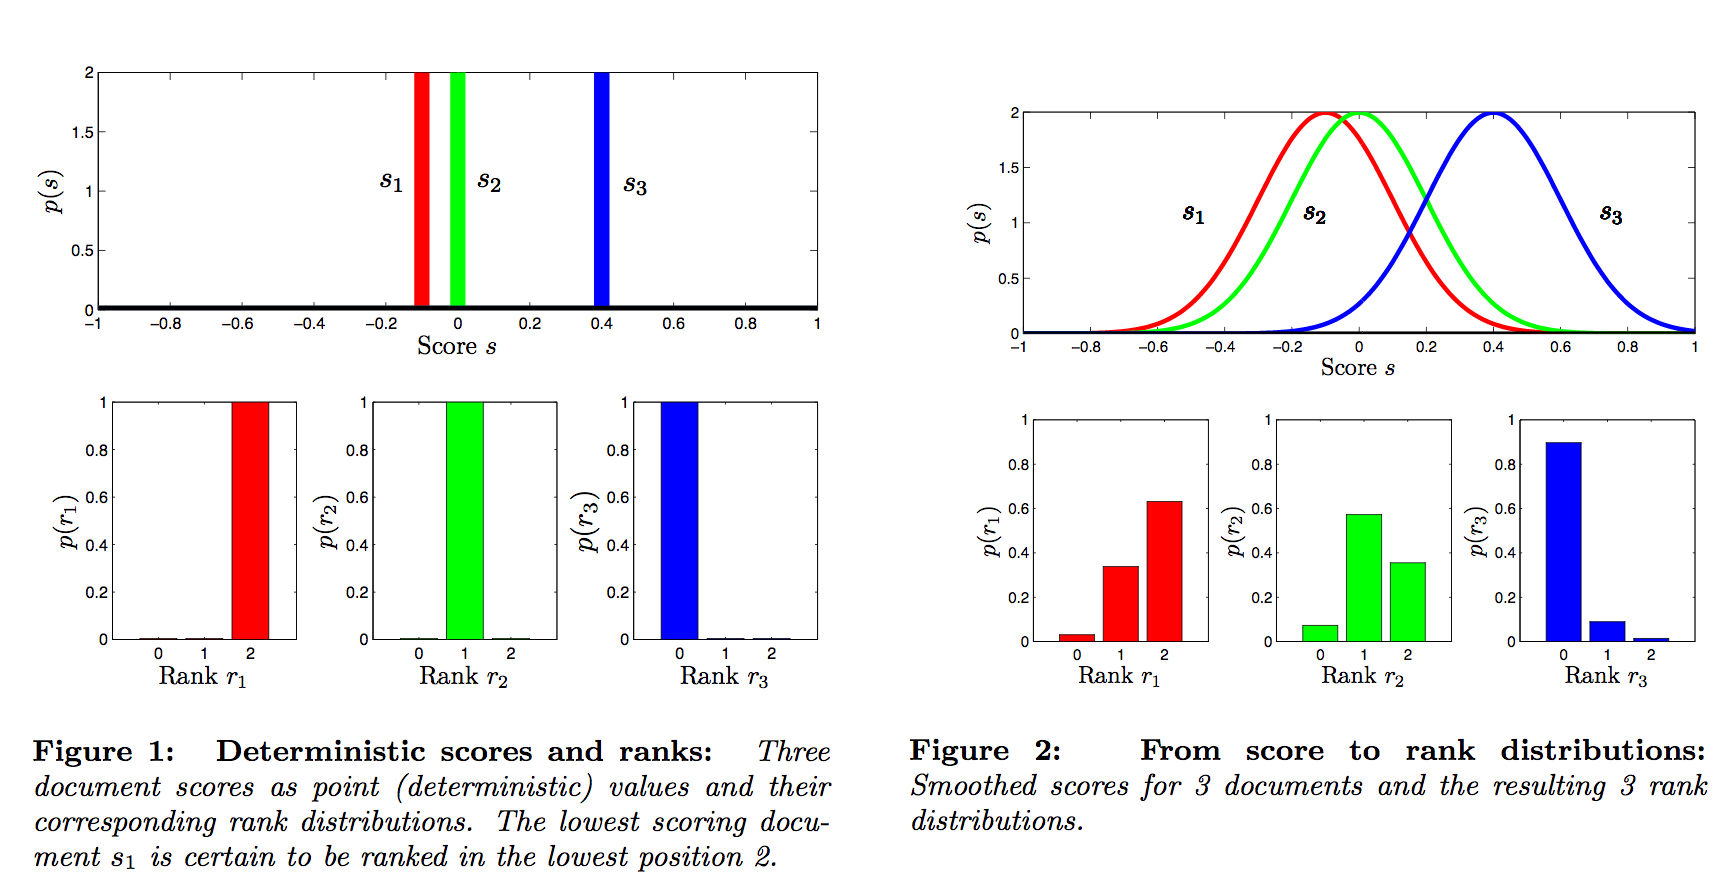
\includegraphics[width=\textwidth]{SoftDCG} \\

Метрика SoftDCG предполагает следующее: вместо того, чтобы каждому документу сопоставлять конкретное место в поисковой выдаче, можно сопоставить ему нормальное распределение на скорах. Т.е. $\t{doc}_i$ имеет скор $t_i$ из распределения $t_i \sim \N(s_i, \sigma^2)$, где $\sigma$ - гиперпараметр.\\
В такой модели $$\pi_{ij} := P(doc_i \t{ выше } doc_j) = P(t_i - t_j > 0) = \Int_{-\infty}^{\infty}\N(x|s_i - s_j,2\sigma^2) dx$$

Из этого выводятся распределения на местах для каждого документа. При этом можно посчитать ожидаемую позицию документа: $$\overset{-}{pos}(j) = \Sum_{i=1,i \neq j}^n \pi_{ij}$$ 

На этом строится подсчет среднего дискаунта каждого документа: $$\hat{d}(j) = \Sum_{i=1}^n p_j(i) \t{discount}(i) - \t{средний дискаунт j-го документа}$$

Далее средние дискаунты используются при подсчете SoftDCG: $$\t{SoftDCG} = \Sum_{i=1}^n \hat{d}_j \cdot r_j$$

\subsection{Свойства метрики}

В то же самое время есть основания полагать, что данная метрика является не совсем <<честной>>, т.к. средняя позиция документа вычисляется, как мат ожидание числа документов выше. Правильный способ подсчета средней позиции документа делается через введение вероятностного распределения на перестановках документов. Описанные в следующих разделах метрики по разному оценивают среднюю позицию документа.

% ============================================================================================================

\newpage
\section{Метрика NoisedSoftDCG}

Рассмотрим другую метрику (назовем ее NoisedSoftDCG). Идея данной метрики берет свое начало в статье про SoftDCG, однако способ подсчета данной метрики несколько иной. \\

\subsection{Описание метрики}

В SoftDCG каждому документу сопоставлялось некоторое вероятностное распределение на множестве возможных занимаемых позиций. При этом следует отметить, что данное распределение вполне четко задавалось аналитически. Благодаря этому имелась возможность задать такой параметр, как $\hat{d}(j)$ (средний дискаунт), формулой. \\

В данном же случае при подсчете метрики принимается во внимание лишь тот факт, что при небольшом изменении скоров на случайные величины значение метрики может меняться в силу того, что близкие документы будут переставляться местами. \\

Алгоритм подсчета NoisedSoftDCG следующий:

\begin{enumerate}
\item Получим скоры ранжирующего алгоритма $s_1,\dots,s_n$
\item Сгенерируем случайный шум $\xi_1,\dots,\xi_n \sim \N(0,\sigma)$
\item $\hat{s}_1=s_1 + \xi_1,\dots,\hat{s}_n=s_n + \xi_n$
\item Посчитаем значение метрики $\t{Value}_{DCG}$
\item Повторим шаги (2)-(4) достаточно большое количество раз (T) и вычислим 
$NoisedDCG = \Sum_{i=1}^T \t{Value}_{DCG}^i$
\end{enumerate}

\subsection{Свойства метрики}

Можно дать некую интуицию по поводу того, почему метрика считается именно так. При достаточно большом Т близкие документы будут часто меняться местами, а усреднение DCG при этом даст некий аналог среднего дискаунта. Таким образом ожидается, что при больших Т данная метрика будет вести себя хорошо в плане гладкости  


% ============================================================================================================

\newpage
\section{Метрика FairSoftDCG}

Еще один вариант метрики, идея которой схожа с NoisedDCG. Заметим, что, основываясь на скорах, выданных ранжирующим алгоритмом, можно ввести вероятностное распределение на перестановках всех документов. \\

\subsection{Описание метрики}

При этом распределение вводится так, что 
$P(d_i \t{ выше } d_j) \sim \frac{e^{\sigma s_j}}{e^{\sigma s_i} + e^{\sigma s_j}}$ (данное распределение можно ввести единственным образом). Благодаря этому для каждой перестановки на документах $\pi_1,\dots,\pi_n$ можно посчитать ее вероятность.

\begin{claim}
Вероятностное распределение на перестановках однозначно задается вероятностями для всех пар документов и задается формулой:
$$P(\pi_1,\dots,\pi_n) = \prod\limits_{i=1}^{n - 1} \frac{e^{\sigma s_{\pi_i}}}{\Sum_{k=j}^n e^{\sigma s_{\pi_j}}}$$
\end{claim}

\begin{theoremproof}
Рассмотрим следующую модель: для построения поисковой выдачи делается n шагов, на k-м из которых выбирается один из оставшихся $n - k + 1$ документов, причем вероятность выбора каждого документа на данном шаге зависит только от тех документов, которые остались. \\

При этом можно заметить, что из парных вероятностей следует то, что вероятность выбора конкретного документа $i$ на данном шаге пропорциональна $e^{\sigma s_i}$. Остается только нормировать эти вероятности на 1. Для этого надо поделить все вероятности на $\Sum_{i = k}^n e^{\sigma s_{j_i}}$ - т.е. на сумму экспонент скоров оставшихся документов.

\end{theoremproof}

Теперь перебрав все перестановки документов можно посчитать <<честное>> мат. ожидание DCG. Собственно это у будет значением FairSoftDCG.
$$FairSoftDCG = \Sum_{\pi} P(\pi_1,\dots,\pi_n) \cdot DCG(\pi_1,\dots,\pi_n)$$

\subsection{Свойства метрики}

При этом возникает ряд проблем с данной метрикой, т.к. вычислительно данная задача достаточно сложная (всего имеется $n!$ возможных перестановок). В связи с этим был выбран способ подсчета близкого к данной метрике значения - подсчета по топ-k документам:
$$FairSoftDCG = \Sum_\pi P(\pi_1,\dots,\pi_k) \cdot DCG(\pi_1,\dots,\pi_k),$$ где сумма берется по всем возможным размещениям по k из n элементов. k берется таким, чтобы метрику можно было посчитать, т.к. n большое и перебор $n!$ перестановок - долгая операция.


% ============================================================================================================

\newpage
\section{Применение результатов}

В данной части будут приведены предполагаемые способы использования искомой метрики. На данный момент идеальной - т.е. гладкой и хорошо аппроксимирующей DCG - метрики не найдено. \\

Итак. Первый и способ применения более гладкой метрики - это использование ее в качестве инструмента показывающего качество обучения модели. Благодаря большей чувствительности появляется возможность следить за тем, как малые изменения гиперпараметров влияют на качество модели.

Простой пример: благодаря этой метрики можно достаточно хорошо измерять влияние новых элементов ансамбля в моделях градиентного бустинга. Точно так же можно использовать данную метрику для active learning like задач. Благодаря высокой чувствительности можно будет немного дообучать алгоритм на небольших частях датасета и смотреть на изменение качества ранжирования. \\

Второй и, пожалуй, важный с практической точки зрения способ применения нашей метрики - смешивание нескольких моделей ранжирования. В наши дни в ранжирующих системах крупных компаний используются абсолютно разные по характеру формулы. Эти формулы имеют разный масштаб выдаваемых значений. Каждая из этих формул придумывалась для оптимизации конкретной метрики - причем метрики могут быть кардинально различными по смыслу. При этом хотелось бы уметь смешивать формулы, выданные несколькими различными моделями, в один ансамбль формул, получая таким образом более мощную формулу ранжирования.

Т.к. наша метрика является гладкой и хорошо аппроксимирует DCG, оптимальная комбинация формул согласно этой метрике должна быть в той же окрестности, что и оптимум с точки зрения DCG. В то же самое время естественно ожидать, что при взятии выпуклой комбинации двух формул должна получаться некая выпуклая гладкая кривая для значений метрики. \\

В качестве своеобразной sanity-check - добавления шума к скорам ранжирующего алгоритма. Здесь имеется ввиду следующее: если добавить к скорам модели шум с неким коэффициентом, это эквивалентно смешиванию двух моделей - нормальной и абсолютно бесполезной. Логично полагать, что оптимум качества в данном случае будет при коэффициенте, с которым берется шум, равном 0 (или близком к 0).

% ============================================================================================================

\newpage
\section{Эксперименты}

\subsection{Зависимость гладкости от размера пула запросов}

Первый эксперимент является одновременно способом проверить наш метод измерения гладкости на адекватность и способом сравнения между собой рассмотренных ранее метрик ранжирования. Здесь и далее рассуждения будут вестись для метрики DCG, но они точно так же верны для любой метрики из списка SoftDCG, NoisedSoftDCG, FairSoftDCG.\\

Для начала вспомним, что такое в нашей задаче <<размер пула>>. Размер пула - это количество обрабатываемых поисковых запросов. Для каждого запроса мы считаем значение DCG, а потом производим усреднение данного значения по всем запросам. Все это происходит при каком-то зафиксированном наборе гиперпараметров.\\

\incpic{paper_decrease_smoothness}
\incpic{noised_decrease_smoothness}

Таким образом для каждого значения набора мы получаем какое-то значение метрики. Например, можно смотреть на значение метрики для ранжирующего алгоритма, который является выпуклой комбинацией двух других алгоритмов, в зависимости от коэффициента, с которым алгоритмы смешиваются. Если рассматривать данный график, на множестве коэффициентов $[0;1]$, можно посчитать его гладкость. При этом, рост размера пула - т.е. увеличение количества запросов, по которому мы усредняем ответ, должно играть роль сглаживающего фактора. \\

Данный эксперимент состоял в том, чтобы посмотреть на изменение гладкости с увеличением роста пула. Хочется заметить, что т.к. увеличивать пул мы возможности не имели, делалось эквивалентное действие - его уменьшение. Ожидалось, что для каждой метрики будет получен график, имеющий обратную пропорциональность - чем больше размер пула, тем меньше ошибка гладкости.\\

На графиках для сравнения приведена гладкость DCG и гладкость соответствующих метрик. Можно заметить, что при некоторых $\sigma$ гладкость нашей метрики значительно лучше (по сравнению с DCG). Также видно, что NoisedSoftDCG - более гладкая, чем PaperSoftDCG.\\

% ============================================================================================================

\subsection{Зависимость качества аппроксимации от размера пула запросов}

Аналогично предыдущему эксперименту логично было бы ожидать графики, на которых с увеличением размера пула ошибка аппроксимации DCG уменьшается. \\

\incpic{dcg_approximation}

Что же касается аппроксимации DCG, можно заметить, что NoisedSofDCG и здесь ведет себя лучше. 

% ============================================================================================================

\subsection{Изменение метрики при добавлении шума}

Как упоминалось ранее, первоочередным действием в работе было желание убедиться в том, что метрика гладкости действительно несет ту смысловую нагрузку, которая на нее была возложена. Для этого проводился эксперимент по смешиванию двух ранжирующих формул, одна из которых была настоящей, а вторая - просто сгенерированным случайным шумом.

\incpic{noised_metrics}

По оси x отложен коэффициент, с которым прибавляется случайный шум, по оси y - значения метрики. Можно заметить, что наши метрики убывают почти монотонно. \\

На графике для каждой метрики показана точка, в которой значение метрики выходит из доверительного интервала (ширина доверительного интервала пропорциональна разности значений метрики в крайних точках). Благодаря этому можно судить о чувствительности метрик: лучше всего добавление плохой модели чувствует SoftDCG, хуже всего - FairSoftDCG. При этом все метрики чувствуют плохую модель лучше, чем оригинальная DCG. Данное свойство важно для использования метрики, как способа контролировать переобучение модели. \\

Подобное поведение в данном эксперименте является необходимым условием для класса искомых метрик.

% ============================================================================================================

\subsection{Изменение метрики для комбинации двух формул}

Самый важный с точки зрения практического применения эксперимент - эксперимент по смешиванию двух формул ранжирования. Цель эксперимента - проверить, какая из наших метрик лучше отображает реальный оптимум качества при использовании в качестве ранжирующей формулы выпуклую комбинацию двух формул.

\incpic{fair_formula_mix}
\incpicture{noised_formula_mix}
\incpicture{paper_formula_mix}

% ============================================================================================================

\newpage
\section{Проблема выбора гиперпараметра}

Так как главной целью работы было получение гладкой метрики, с помощью которой можно будет удобно и правильно подбирать коэффициенты в смеси ранжирующих формул, остановимся на этом эксперименте. \\

Как можно было заметить из графиков, приведенных выше, при разных значениях гиперпараметра $\sigma$ получаются разные качества аппроксимации/гладкости. При этом, логично предположить следующее: чем лучше аппроксимация (т.е. чем ближе $\sigma$ к 0), тем хуже гладкость кривой. Ниже приведен график в осях, соответствующих данным двум показателям, метрик с разными гиперпараметрами.

\incpic{tradeoff_max_min}

Как видно из графика, для каждой метрики в можно варьировать этот гиперпараметр, получая тем самым желаемый компромисс между гладкостью метрики и хорошей аппроксимацией DCG. \\

Следует отметить, что выбор параметра - неочевидная задача. В итоге, возникает проблема определения $\sigma$. Она заключается в том, что необходимо выбирать данный параметр, опираясь, лишь на скоры, выданные каждой из формул. Однако скоры в каждом запросе свои. В добавок функция, которую мы при этом пытаемся минимизировать: 
\i{$\alpha \cdot \t{approx} + \beta \cdot \t{smoothness}$}, не является гладкой  относительно $\sigma$. \\

Данную проблему можно описать следующим образом. Представим себе смесь двух формул ранжирования, где вторая формула совпадает в первой, но выдает значения в 10 раз больше. Очевидно вторая формула более устойчива к добавлению шума. Таким образом, даже если вторая формула хуже, наша метрика может предпочитать отдавать ей больший коэффициент в выпуклой комбинации потому, что выбрана слишком большая $\sigma$. При этом, если есть две разные формулы, значения которых нормированы на [0;1], может оказаться, что одна значительно лучше устойчива к шуму, нежели вторая - но при этом нам хотелось бы понимать, что в смеси формул лучше отдавать предпочтение первой. \\

Также можно рассмотреть графики зависимости ошибок гладкости и аппроксимации от размера пула. Видно, что для каждой метрики данные ошибки сначала убывают с увеличением $\sigma$, а потом возрастают. При этом выбор $\sigma$ для которой они будут оптимальны в применении к конкретным формулам ранжирования неочевиден. \\

Есть некоторые эвристики по подбору $\sigma$, но хорошего решения в ходе исследования данного вопроса найдено не было.

% ============================================================================================================

\newpage
\section{Выводы}

В ходе исследования была рассмотрена реализация метрики SoftDCG, идея которой описана в \cite{SoftDCGPaper}. Также были рассмотрены предложенные автором аналоги этой метрики: NoisedSoftDCG и FairSoftDCG. \\

При изучении этих метрик были введены такие параметры, как <<гладкость>> и <<аппроксимация DCG>>. Было проведено исследование касательно изменения этих показателей при изменении различных гиперпараметров. Это дало возможность понять, что представленные метрики в целом являются неким продвижением в нужном направлении - но окончательного решения не дают. \\

По результатам исследования автор отдает предпочтение метрике NoisedSoftDCG, т.к. в экспериментах она показала себя лучше. Ошибки гладкости и аппроксимации данной метрики меньше, чем у SoftDCG. При этом сложно проводить хорошее сравнение с FairSoftDCG в силу того, что она является вычислительно сложной. Важным свойством NoisedSoftDCG является также то, что при уменьшении размера пула почти в 2 раза мы можем значительно не терять в гладкости и аппроксимации DCG - чего нельзя сказать о SoftDCG. \\

Важный вывод можно сделать из эксперимента со смешиванием двух формул ранжирования: лучше всего себя в данном случае ведет FairSoftDCG - что совпадает с идеей ее конструкции (это <<честный>> способ считать SoftDCG). При этом можно заметить, что NoisedDCG показала себя лучше в данном эксперименте при меньших $\sigma$ - для данной метрики важен параметр T (количество усреднений). При слишком больших $\sigma$ и малых T шум слишком сильно влияет на метрику, и она приближается к константе.

\begin{tabular}{|c|c|c|c|c|}
\hline
\t{Метрика} & $\sigma$ & $\t{err}_\t{smooth}$ & $\t{err}_\t{approx}$ & $\frac{\t{err}_\t{smooth}}{5} + \t{err}_\t{approx}$ \\
\hline
FairSoftDCG & 0.5 & 59.381 & 1.729 & 13.605 \\
\hline
FairSoftDCG & 1 & 54.400 & 3.663 & 14.543 \\
\hline
NoisedDCG & 0.5 & 47.903 & 1.667 & 11.248 \\
\hline
NoisedDCG & 1 & 37.492 & 11.960 & 19.584 \\
\hline
SoftDCG & 0.5 & 56.461 & 7.285 & 18.577 \\
\hline
SoftDCG & 1 & 53.389 & 3.091 & 13.769 \\
\hline
\end{tabular} \\

Была исследована проблема выбора гиперпараметра $\sigma$, который соответствует тому, насколько сильно наша метрика стремится раздвинуть между собой документы (фактически - порядок разницы между скорами близких документов). 

% ============================================================================================================

\newpage

\begin{thebibliography}{1}

\bibitem{SoftDCGPaper} \href{https://www.microsoft.com/en-us/research/publication/softrank-optimising-non-smooth-rank-metrics/}
{M. Taylor, J. Guiver, S. Robertson and T. Minka. SoftRank: Optimising Non-Smooth Rank Metrics. Microsoft Research Cambridge, 2016}

\bibitem{LambdaMARTPaper} \href{https://www.microsoft.com/en-us/research/publication/from-ranknet-to-lambdarank-to-lambdamart-an-overview/}
{Christopher J.C. Burges. From RankNet to LambdaRank to LambdaMART. Microsoft Research Technical Report, 2010}

\bibitem{LearningToRankPaper} \href{https://www.microsoft.com/en-us/research/publication/learning-to-rank-from-pairwise-approach-to-listwise-approach/}
{Zhe Cao, Tao Qin, Tie-Yan Liu, Ming-Feng Tsai, Hang Li. Learning to Rank: From Pairwise Approach to Listwise Approach. Microsoft Research Technical Report, 2007}

\end{thebibliography}

\vspace{0.7cm}

\section*{Appendix}

\subsection*{SoftDCG code}
\lstinputlisting[language=Python, breakatwhitespace=true, breaklines=true, commentstyle=\color{blue}]{soft_code.py}

~\\

\subsection*{NoisedSoftDCG code}
\lstinputlisting[language=Python, breakatwhitespace=true, breaklines=true, commentstyle=\color{blue}]{noised_code.py}

~\\

\subsection*{FairSoftDCG code}
\lstinputlisting[language=Python, breakatwhitespace=true, breaklines=true, commentstyle=\color{blue}]{fair_code.py}

~\\

\subsection*{SmoothnessError code}
\lstinputlisting[language=Python, breakatwhitespace=true, breaklines=true, commentstyle=\color{blue}]{smoothness_code.py}

~\\

\subsection*{ApproximationError code}
\lstinputlisting[language=Python, breakatwhitespace=true, breaklines=true, commentstyle=\color{blue}]{approximation_code.py}

\end{document}
